\chapter{Internet des objets}
	
	
	\section{Introduction}
	Le concept  d’Internet des Objets (IoT pour Internet of Things en anglais) a été proposé en 1999 par le laboratoire Auto-ID du Massachusetts Institute of Technology (MIT) \cite{hu2016security}.\\ 

	Imaginez un monde où des milliards d'objets peuvent détecter, communiquer et partager des informations, tous interconnectés via des réseaux IP (Internet Protocol) publics ou privés. Ces objets interconnectés ont des données régulièrement collectées, analysées et utilisées pour initier l'action, fournissant une richesse d'intelligence pour la planif{\kern0pt}ication, la gestion et la prise de décision \cite{patel2016iot}. C'est le monde de l'Internet des objets (IoT).\\
	
	Un exemple de base de tels objets comprend les thermostats et les systèmes de surveillance et de contrôle HVAC (chauf{\kern0pt}fage, ventilation, climatisation) qui forment les composants des maisons intelligentes. Il existe également d’autre domaines et environnements dans lesquels l’IoT peut jouer un rôle remarquable et améliorer la qualité de nos vies. Ces applications comprennent soins de santé, transports, automatisation industrielle et réponse d'urgence aux catastrophes naturelles et d'origine humaine dont la prise de décision humaine est dif{\kern0pt}f{\kern0pt}icile.\\
	
	L'idée de base de ce concept d’IoT est la présence omniprésente autour de nous d'une variété de choses ou d'objets - tels que des réseaux Wi-Fi, des réseaux cellulaires, des étiquettes d'identif{\kern0pt}ication par radiofréquence (RFID pour Radio Frequency Identif{\kern0pt}ication), des capteurs, des actionneurs, des téléphones mobiles, etc. - qui, grâce à des schémas d'adressage uniques, sont capables interagir entre eux et coopérer avec leurs voisins pour atteindre des objectifs communs \cite{atzori2010iot}.\\
	
	Dans ce chapitre, nous présentons l’Internet des Objets, l’origine de son concept, ses caractéristiques diverses. Puis on illustre ses dif{\kern0pt}férentes architectures, ses domaines d’application où il introduit de l’intelligence, ainsi que les enjeux et les déf{\kern0pt}is que l’on peut rencontrer aux objets connectés.
	
		
	\section{Historique}
	Le premier \og objet \fg{}  connecté à l’Internet à utiliser ce nouveau protocole a été un grille-pain. En 1990, John Romkey, ingénieur logiciel et premier évangéliste d'Internet, en avait construit un qui pourrait être allumé et éteint sur Internet. Romkey a laissé tomber quelques tranches de pain dans le grille-pain et, à l'aide d'un ordinateur maladroit, a allumé le grille-pain. Il faudra encore une décennie avant que quiconque utilise l'expression « Internet des objets », mais le petit grille-pain magique de Romkey montre à quoi pourrait ressembler un monde d'objets connectés à Internet \cite{pardes2020iot}.\\
	 
	Le terme « Internet of Things » lui-même a été inventé en 1999 dans le laboratoire Auto-ID du MIT lorsque le britannique Kevin Ashton (pionnier de la technologie) l'a mis dans une présentation pour l’entreprise Procter \& Gamble. Le terme « Auto-ID » fait référence à toute grande classe de technologies d'identif{\kern0pt}ication utilisées dans l'industrie pour automatiser, réduire les erreurs et augmenter l'ef{\kern0pt}f{\kern0pt}icacité. Ces technologies comprennent les codes à barres, les cartes à puce, les capteurs, la reconnaissance vocale et la biométrie \cite{sundmaeker2010vision}. Ashton, qui travaillait alors dans l'optimisation de la chaîne d'approvisionnement, a remarqué que l'optimisation dépend directement de la vitesse de transmission et de traitement des données. Cela peut prendre des jours pour les personnes qui collectent les données. De plus, conf{\kern0pt}ier la tâche à des ordinateurs n’était pas envisageable car dépourvus d’organes sensoriels, ils étaient dépendants des informations que des opérateurs humains voulaient bien leur fournir. L'utilisation de l'identif{\kern0pt}ication par radiofréquence (RFID) a permis d'accélérer le processus de transfert de données directement entre les appareils. Il avait une idée des choses à collecter, traiter et transmettre sans intervention humaine.\\

	Alors qu’à domicile l'internet est devenu omniprésent et que le Wi-Fi s'est accéléré, le rêve de la maison intelligente a commencé à ressembler davantage à une réalité. Les entreprises ont commencé à présenter de plus en plus de ces inventions: des cafetières « intelligentes », des fours qui préparent des biscuits avec un minutage précis et des réfrigérateurs qui ont automatiquement réapprovisionné le lait périmé. Le premier d'entre eux, le réfrigérateur connecté à Internet de LG, a été lancé sur le marché en 2000. Il pourrait faire le point sur le contenu des étagères, et les dates d'expiration.

\begin{table}[H]
	\begin{center}
	\begin{tabular}{|p{3cm}|p{8cm}|}
	\hline 
	\multicolumn{2}{|c|}{\textbf{Internet des objets au f{\kern0pt}il des années}} \\ 
	\hline 
	1990 & John Romkey crée le premier appareil IoT: un grille-pain qu'il contrôle avec son ordinateur \\ 
	\hline 
	1999 & Kevin Ashton invente le terme « Internet des objets » pour décrire un système où Internet est connecté au monde physique via des capteurs omniprésents \\ 
	\hline 
	2000 & LG présente son premier réfrigérateur connecté avec un prix de 20 000 \$ \\ 
	\hline 
	2008 & La première conférence Internet des Objets au monde se tient à Zurich, en Suisse \\ 
	\hline 
	2010 & Tony Fadell fonde Nest, qui développe des appareils électroménagers intelligents et des systèmes de gestion des bâtiments. \\ 
	\hline 
	2013 & Oxford Dictionary ajoute le terme « Internet of Things » \\ 
	\hline 
	2014 & Amazon présente le haut-parleur Echo, ainsi que l'assistant vocal Alexa, une nouvelle façon de contrôler la maison intelligente \\ 
	\hline 
	2016 & Un logiciel malveillant appelé Mirai a exploité des vulnérabilités dans plus de 600000 appareils IoT pour créer une attaque massive par déni de service distribué (\textbf{DDoS}). \\ 
	\hline 
	2020 & Selon certaines estimations, le nombre d'appareils connectés à Internet dépasse 20 milliards. Et les prévisions suggèrent que d'ici 2030, environ 50 milliards de ces appareils IoT seront utilisés dans le monde \cite{statista2020iot}.
	 \\ 
	\hline 
	\end{tabular} 
	\end{center}
	\caption{Internet des Objets au f{\kern0pt}il des années}
\end{table}

	\section{Déf{\kern0pt}inition}
	Le Cluster des projets européens de recherche sur l'Internet des objets (CERP-IoT pour Cluster of European Research Projects on the Internet of Things) déf{\kern0pt}init l’Internet des objets comme : « une infrastructure dynamique d’un réseau global. Ce réseau global a des capacités d’auto-conf{\kern0pt}iguration basée sur des standards et des protocoles de communication interopérables. Dans ce réseau, les objets physiques et virtuels ont des identités, des attributs physiques, des personnalités virtuelles et des interfaces intelligentes, et ils sont intégrés au réseau d’une façon transparente » \cite{sundmaeker2010vision}.\\
Cette vision de l’Internet des objets introduira une nouvelle dimension aux technologies de l’information et de la communication : en plus des deux dimensions temporelle et spatiale qui permettent aux personnes de se connecter de n’importe où à n’importe quel moment, nous aurons une nouvelle dimension « objet » qui leur permettra de se connecter à n’importe quel objet \cite{challal2012securite} (Smartphone, tablettes, capteurs, caméras de vidéosurveillance, etc.). Un objet connecté a une valeur lorsqu’il est connecté à d’autres objets et consorts logiciels, par exemple : une montre connectée n’a d’intérêt qu’au sein d’un écosystème orienté santé/bien-être, qui va bien au-delà de connaître l’heure.\\

	L’Internet des Objets a pour but de permettre aux objets d’être connecté à tout moment, en tout lieu, avec n’importe quoi et n’importe qui en utilisant n’importe quel chemin / réseau et n’importe quel service \cite{patel2016iot}.\\
	
	\begin{figure}[H]
		\begin{center}
			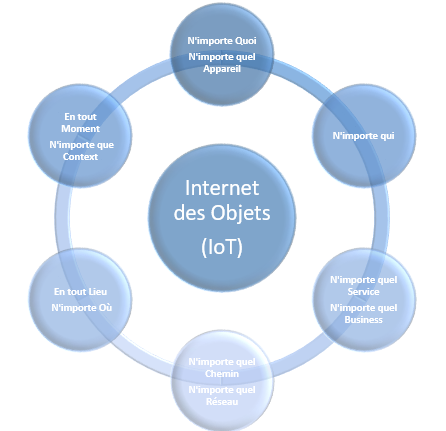
\includegraphics{IMAGES/ORIGINALS/Internet_des_Objets}
		\end{center}
		\caption{Internet des Objets}
	\end{figure}

\textbf{L’Internet des Objets} peut être déf{\kern0pt}ini également comme « des données et des appareils disponibles en permanence à travers l’internet » \cite{hu2016security}.\\

\textbf{Un objet connecté} est un objet possédant la capacité d’échanger des données avec d’autres entités physiques ou numériques.\\

À peu près n'importe quel objet physique peut être transformé en un appareil IoT s'il peut être connecté à Internet pour être contrôlé ou communiquer des informations avec le réseau indépendamment de l’action humaine.\\

Pour illustrer, prenons un exemple dans le domaine de l’habitat intelligent, aussi connu sous le nom de Smart Home. Imaginez que votre réfrigérateur devienne intelligent. Un réfrigérateur capable de vous dire en temps réel le type de denrées qu’il y a à l’intérieur et capable de passer commande pour vous quand vous avez besoin de vous réapprovisionner.

Le réfrigérateur est un exemple typique mais le nombre d’objets qu’il est aujourd’hui possible de connecter pour s’échanger des données est illimité.\\

	\begin{figure}[H]
		\begin{center}
			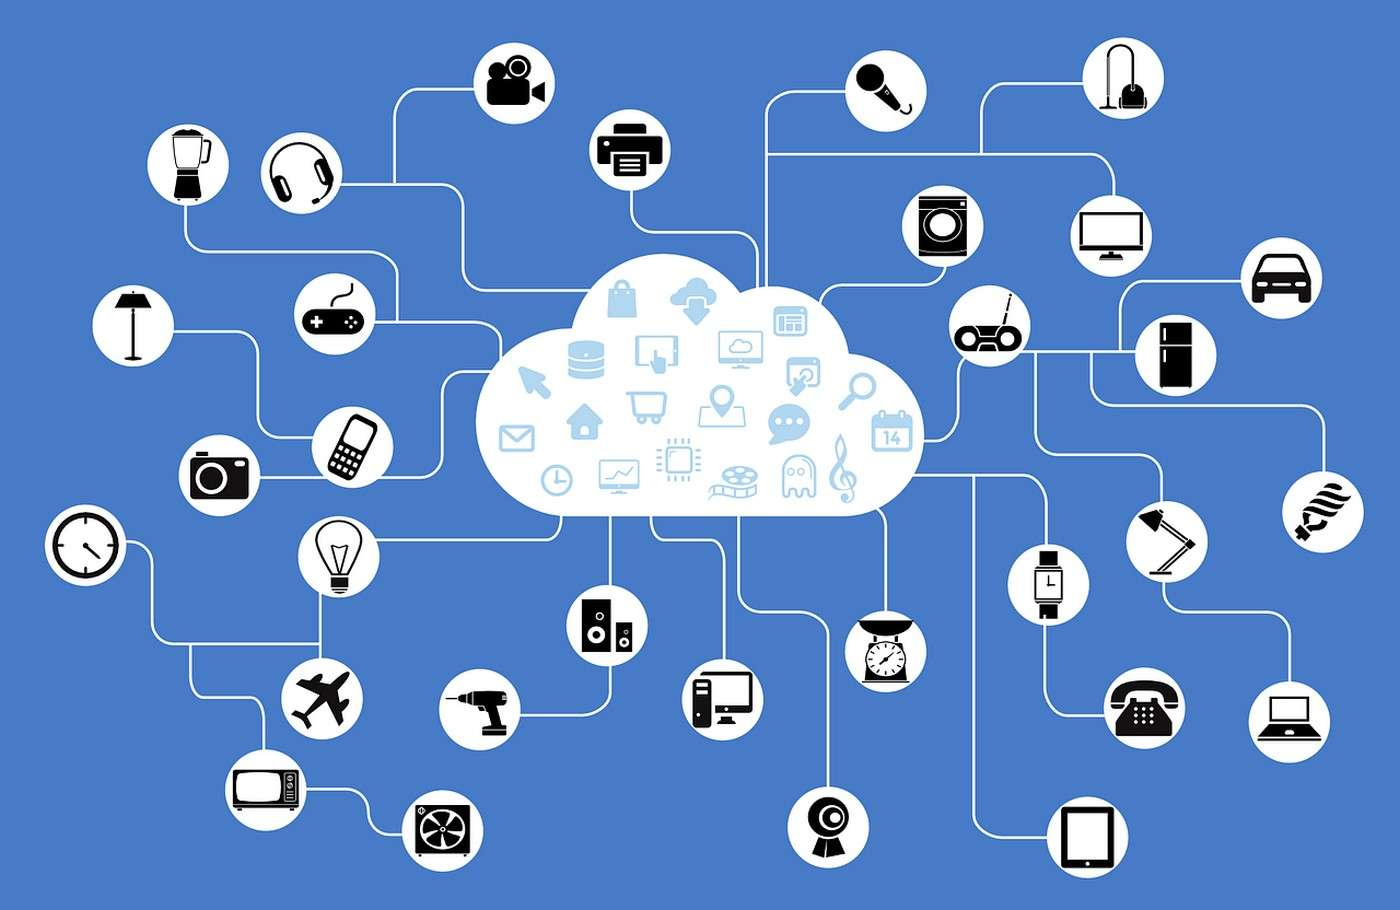
\includegraphics[width=16cm,height=14cm]{IMAGES/ORIGINALS/Internet_des_Objets_2}
		\end{center}
		\caption{Internet des Objets}
	\end{figure}
	
	
	\section{Caractéristiques}
	Les caractéristiques fondamentales de l'IoT sont les suivantes \cite{patel2016iot,vermesan2014iot}:\\
	
	\textbf{Inter connectivité}: en ce qui concerne l'IoT, tout peut être interconnecté avec l'infrastructure mondiale d'information et de communication.\\
	
	\textbf{Services liés aux objets}: l'IoT est capable de fournir des services liés aux objets dans les limites des objets, tels que la protection de la vie privée et la cohérence sémantique entre les objets physiques et les objets virtuels associés. Af{\kern0pt}in de fournir des services liés aux objets dans les contraintes des objets, les technologies du monde physique et du monde de l'information vont changer.\\
	
	\textbf{Hétérogénéité}: les appareils de l'IoT sont hétérogènes car basés sur dif{\kern0pt}férentes  plates-formes matérielles et réseaux. Ils peuvent interagir avec d'autres appareils ou plates-formes de services via dif{\kern0pt}férents réseaux.\\

	\textbf{Changements dynamiques}: l'état des appareils change de manière dynamique, par exemple, le sommeil et le réveil, connectés et / ou déconnectés ainsi que le contexte des appareils, y compris l'emplacement et la vitesse. De plus, le nombre d'appareils peut changer dynamiquement.\\
	
	\textbf{Échelle énorme}: le nombre d'appareils qui doivent être gérés et qui communiquent entre eux sera au moins d'un ordre de grandeur supérieur à celui des appareils connectés à l'Internet actuel. Encore plus critique sera la gestion des données générées et leur interprétation à des f{\kern0pt}ins d'application. Cela concerne la sémantique des données, ainsi que la gestion ef{\kern0pt}f{\kern0pt}icace des données.\\
	
	\textbf{Sécurité}: à mesure que nous tirons parti de l'IoT, nous ne devons pas oublier la sécurité. En tant que créateurs et destinataires de l'IoT, nous devons concevoir pour la sécurité. Cela comprend la sécurité de nos données personnelles et la sécurité de notre bien-être physique. Sécuriser les points de terminaison, les réseaux et les données se déplaçant sur tout cela signif{\kern0pt}ie créer un paradigme de sécurité qui évoluera.\\
	
	\textbf{Intelligence} : L'IoT est livré avec la combinaison d'algorithmes et de calcul, de logiciels et de matériel qui le rendent intelligent. Ce qui le rend encore plus intelligent, ce sont les données qu’il recueille à travers un capteur. L'intelligence ambiante dans l'IoT améliore ses capacités qui facilitent les choses pour répondre de manière intelligente à une situation particulière et les aide à ef{\kern0pt}fectuer des tâches spécif{\kern0pt}iques. Malgré toute la popularité des technologies intelligentes, l'intelligence dans l'IoT ne concerne que les moyens d'interaction entre les appareils, tandis que l'interaction utilisateur et appareil est obtenue par des méthodes d'entrée standard et une interface utilisateur graphique.\\
	
	\textbf{Connectivité}: la connectivité permet l'accessibilité et la compatibilité du réseau. L'accessibilité se fait sur un réseau tandis que la compatibilité of{\kern0pt}fre la capacité commune de consommer et de produire des données.


	\section{Architecture de l’IoT}	
	L’IoT devrait être capable d’interconnecter des milliards d’objets hétérogènes via le réseau internet, ainsi il est judicieux d’adopter une architecture flexible.\\
	
Le modèle de base est une architecture à trois-couches comportant les couches Application, Réseau, et Perception. D’autres modèles ont été proposé récemment qui ajoutent plus d’abstraction aux architectures des objets connectés. La f{\kern0pt}igure ci-dessous illustre les dif{\kern0pt}férentes catégories de l’architecture IoT \cite{al2015iot}.\\

	\begin{figure}[H]
		\begin{center}
			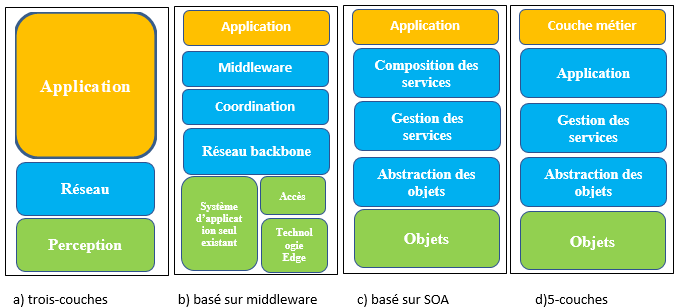
\includegraphics[width=\textwidth]{IMAGES/ORIGINALS/diverses_architectures_de_l'IoT}
		\end{center}
		\caption{Diverses architectures de l'IoT}
	\end{figure}


	\subsection{Architecture à trois couches}
	\subsubsection{Couche perception }
La première couche de l’IoT, les Objets (appareils) ou couche perception, est un organe sensoriel de l’IoT, représente les capteurs physiques de l’IoT qui essaie de recueillir et traiter les données. Un capteur de température permet de traduire l’amplitude de la température en une tension électrique. Cette couche comprend principalement des éléments avec des étiquettes RFID, capteurs, et autre terminaux. Elle détecte les données de l’environnement. Certains facteurs sont pris en charge par la couche physique tels que : ressource, hétérogénéité, déploiement, protocoles.\\

	\subsubsection{Couche réseau}
La couche réseau est chargée de récupérer les données collectées du capteur. L’échange des données se fait via cette couche. Ainsi, la couche réseau peut agréger les données dans sa propre base de données ou un stockage cloud.\\

	\subsubsection{Couche application}
La couche application ou la couche interface utilisateur contient les méthodes d’interaction avec les applications de l’utilisateur.\\

	\subsection{Architecture à cinq couches}
	\subsubsection{Couche Objets}
La première couche de l’IoT, les Objets (appareils) ou couche perception, représente les capteurs physiques de l’IoT qui essaie de recueillir et traiter les données. Cette couche comprend les capteurs et les actionneurs qui fonctionnent dif{\kern0pt}féremment. Un capteur de température permet de traduire l’amplitude de la température en une tension électrique. On a d’autres grandeur mesurable tels que pression, luminosité, position, vitesse. Quant aux actionneurs, ils permettent d’agir dans le monde physique en changeant son état. Un actionneur peut allumer un appareil à distance. La couche perception collecte les informations du capteur, numérise et transmet les données à la couche Abstraction Objet via un canal sécurisé.\\

	\subsubsection{Couche Abstraction Objet}
La couche Abstraction Objet transfert les données produit par la couche perception à la couche Gestion Service à travers des canaux sécurisés. Les données peuvent être transféré via des technologies variés tels que RFID, GSM(2G), UMTS(3G), LTE(4G), WI-FI, Bluetooth, Zigbee, etc. En plus, d’autres fonctions comme Cloud Computing et le traitement de gestion de données sont gérés par cette couche.\\

	\subsubsection{Couche Gestion des Services}
La couche Gestion des Services garantit la fourniture des services en fonction de la demande de l'utilisateur dans un environnement réseau hétérogène.

	\subsubsection{Couche Application}
La couche Application fournit les services demandés par les clients. Par exemple, la couche application peut fournir les mesures de température au client qui demande cette information.
Elle couvre dif{\kern0pt}férentes applications, à savoir: ville intelligente, transport intelligent, soins de santé, agriculture intelligente, maison intelligente, etc.\\

	\subsubsection{Couche Business}
La couche métier(gestion) est chargée de gérer l’ensemble des activités et des services comme les modèles métiers. Elle aide à construire un graphique, un organigramme, un modèle métier, une prise de décision etc. basé sur les données reçues de la couche Application.


	\section{Domaines d’application}
Il existe une panoplie de domaines d’application extrêmement diverses pour les secteurs de l’internet des objets, du machine to machine et des objets connectés. Parmi ces principaux domaines, nous citons : la smart city, la domotique, les transports, la santé, l’industrie, l’agriculture.\\

	\begin{figure}[H]
		\begin{center}
			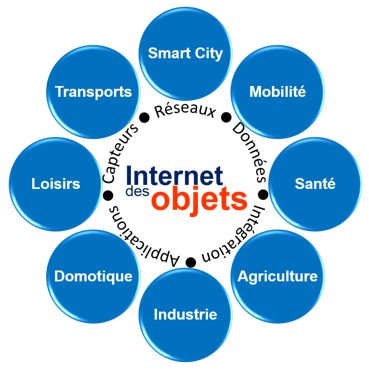
\includegraphics{IMAGES/ORIGINALS/Application_IoT}
		\end{center}
		\caption{Domaines d'application de l'IoT}
	\end{figure}

	\begin{enumerate}
		\item \textbf{Smart city}\\
Dans les villes intelligentes, il améliore la qualité de vie des habitants en utilisant les nouvelles technologies pour accroître l’ef{\kern0pt}f{\kern0pt}icacité des services, optimiser l’éclairage, de maîtriser la consommation d’énergie et de réduire l’impact écologique des activités urbaines.
		\item \textbf{Domotique}\\
		La domotique regroupe l’ensemble des technologies permettant l’automatisation des équipements d’un habitat. Elle vise à apporter des solutions techniques pour répondre aux besoins de confort (gestion d’énergie, optimisation de l’éclairage et du chauf{\kern0pt}fage), de sécurité(alarme) et de communication (commandes à distance) \cite{locqueneux2015domotique}.\\
		La domotique couvre trois domaines principaux :
		\begin{enumerate}
			\item Confort de la vie quotidienne : l’IoT permettra aux propriétaires de villa de déclencher arrosage, fermeture des fenêtres ou tonte du gazon en fonction des informations transmises par les capteurs disposés dans le jardin.
			\item Assurer la protection des personnes et des biens par la prévention des risques d’accident (incendies, fuite de gaz, etc.).
			\item Faciliter les économies d’énergie grâce à la réaction maitrisée d’une maison intelligente.
		\end{enumerate}

		\item \textbf{Santé}\\
		Dans le domaine de la santé, l’internet des objets of{\kern0pt}frira une sécurité accrue à un patient dont un capteur est intégré sur le corps qui donne la possibilité d’être monitoré à distance.\\
Il peut informer un patient quand il est temps de prendre le médicament. En outre, cela pourrait éventuellement informer le médecin d’une situation d’urgence lui permettant ainsi de localiser le patient grâce à l’objet connecté.\\

		\item \textbf{Transport}\\
		Des voitures connectées ou autonomes aux systèmes de transports intelligents, l’IoT pourra sauver des vies, réduire le traf{\kern0pt}ic et minimiser l’impact des véhicules sur l’environnement.
		
		\item \textbf{Industrie}\\
		Dans le secteur industriel, le machine to machine peut augmenter énormément la productivité et la performance d’une usine. Par exemple, supposons un réseau de capteurs polyvalents qui suit à distance et pilote le fonctionnement des machines en leur donnant la possibilité de déclencher elles-mêmes un réapprovisionnement en matières premières.
		
		\item \textbf{Agriculture}\\
		L’internet des objets à un impact énorme sur le domaine de l’agriculture. Les éleveurs en bénéf{\kern0pt}icient en ef{\kern0pt}fectuant un suivi plus précis de l’alimentation, de la santé et de la sécurité du bétail. Ils peuvent aussi géolocaliser leur bétail en temps réel. Les agriculteurs peuvent aussi recueillir des données sur les engrais et les pesticides nécessaires à leurs cultures \cite{krigman2018agriculture}.
	\end{enumerate}
	\newpage
	\section{Enjeux et déf{\kern0pt}is de l’IoT}
	L’internet des objets soulève un nombre important de questions, mais le plus important porte certainement sur la sécurité. Beaucoup de produit connectés, dont certains que nous utilisons au quotidien af{\kern0pt}f{\kern0pt}ichent un réel manque de maturité impliquant de nouvelles préoccupation notamment autour de la conf{\kern0pt}identialité et la sécurité des données.\\
Mirai est un exemple type de cyberattaques résultant de menaces de sécurité liées à l’IoT.

\begin{table}[H]
	\begin{center}
	\begin{tabular}{|p{3cm}|p{10cm}|}
		\hline 
\textbf{Enjeux} & \textbf{Déf{\kern0pt}is} \\ 
		\hline 
Architecture & De nombreux chercheurs ont proposé diverses architectures non encore standardisé. \\ 
		\hline 
Sécurité & L’échange d’information entre des milliards d’objets connecté sur internet se fait via une connexion réseau sans f{\kern0pt}il. \\ 
		\hline 
Conf{\kern0pt}identialité & Les opérations d’accès aux prof{\kern0pt}ils entre objets sans interférences sont dif{\kern0pt}f{\kern0pt}iciles. \\ 
		\hline 
Intéroperabilité & Communication machine à machine (M2M), un déf{\kern0pt}i de l’IoT dû à la nécessité de gérer un grand nombre d’objets hétérogènes qui appartiennent à dif{\kern0pt}férentes plates-formes. \\ 
		\hline 
Disponibilité & La capacité à fournir des services à tout moment, n’importe où et n’importe quoi est un déf{\kern0pt}is. \\ 
		\hline 
Mobilité & L'utilisateur ou les appareils qui se connectent peuvent obtenir les services lors de leurs déplacements, ce qui constitue un déf{\kern0pt}i. \\ 
		\hline 
Scalabilité & La possibilité d'ajouter de nouveaux appareils qui n'af{\kern0pt}fecte pas la qualité de services existent est un déf{\kern0pt}i. \\ 
		\hline 
	\end{tabular} 
	\end{center}
	\caption{Enjeux et déf{\kern0pt}is de l'IoT}
\end{table}
\newpage
	\section{Sécurité, conf{\kern0pt}identialité (privacy) en IoT}
L’IoT nécessite cinq phases, de la collecte des données, du stockage, du traitement, de la transmission des données à la livraison des données aux utilisateurs f{\kern0pt}inaux sur demande ou non \cite{hu2016security}. Les capteurs collectent dans de nombreux cas des données extrêmement sensible (personnelles). En ef{\kern0pt}fet les objets connectés produisent de grandes quantités de données à la phase de collecte de données et le traitement de cette masse de données implique de nouvelles préoccupations notamment autour de la conf{\kern0pt}identialité et la sécurité des données.
	\begin{figure}[H]
		\begin{center}
			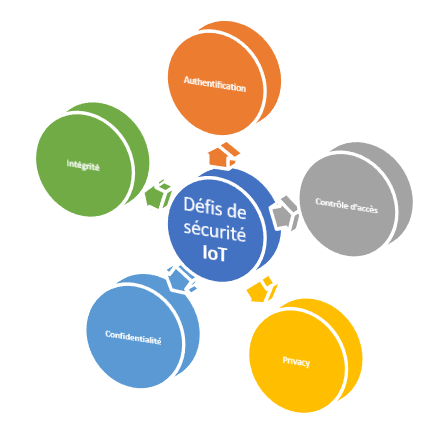
\includegraphics[width=\textwidth]{IMAGES/ORIGINALS/Défis_de_sécurité_IoT}
		\end{center}
		\caption{Déf{\kern0pt}is de sécurité IoT}
	\end{figure}

	\subsection{Sécurité pour l’IoT}
La sécurité est l’af{\kern0pt}faire de tous, elle concerne chacun de nous. Si vous achetez un verrou « intelligent » pour votre porte d’entrée, il est fort probable que vous allez vous faire pirater dans un premier temps puis cambrioler. L’IoT a des avantages et apporte tous celui d’internet à des éléments comme les thermostats et les ampoules par exemple mais sans oublier qu’il apporte également les problèmes d’internet. A présent que les gens ont leur réfrigérateurs, sonnettes, télévisions, ampoules, caméras de sécurité, haut-parleur connectés au Wi-Fi, presque tous les appareils de la maison peuvent être compromis ou rendu inutiles. En ef{\kern0pt}fet les objets connectés peuvent servir de point d’accès à votre réseau avec vos portables, votre PC, bref toute votre vie.\\

La menace qui pèse sur les appareils connectés à Internet ne vient pas uniquement du fait qu’ils sont connectés à Internet, mais aussi parce que les fabricants d’appareils n’ont pas toujours conçu leurs produits en privilégiant la sécurité. À mesure que l'IoT se répand largement, les cyberattaques risquent de devenir de plus en plus physiques (et pas simplement virtuelles) \cite{clearfield2013rethinkingsiot}. Les appareils contrôlés par ordinateur dans les automobiles, tels que les freins, les moteurs, les serrures, les klaxons, les systèmes de chauf{\kern0pt}fage et les tableaux de bord, se sont révélés vulnérables aux attaquants qui ont accès au réseau de bord \cite{andy2013hackers,boyle2010proof}. La possibilité qu'un intrus puisse démarrer à distance le chauf{\kern0pt}fage, régler le climatiseur, déverrouiller les portes, déployer des airbags pendant que vous conduisez sans accident ou tourner le volant d'une voiture en marche est en ef{\kern0pt}fet inquiétante, ef{\kern0pt}frayante.\\

Jusque-là l’essentiel des dommages subit par l’IoT a été causé par les botnets. En septembre 2016, une attaque a été mis en place par des centaines de milliers d’objets connecté piraté pour former un énorme botnet appelé Mirai. Ce malware a exploité des vulnérabilités (que les fabricants d’objet connecté ne prenaient pas en compte) dans plus de 600 000 appareils IoT pour créer une attaque massive par déni de service distribué (\textbf{DDoS}). Il avait pour objectif de dénoncer les risques de l’IoT.\\

En raison de la vulnérabilité du WPA2(protocole qui sécurise les échanges en Wi-Fi), tout ce qui est connecté à un réseau Wi-Fi risque d’être piraté \cite{kasperski201krack}. L'année suivante après Mirai, une attaque appelée KRACK acronyme de Key Reinstallation Attack (attaque de réinstallation de clé) a infecté presque tous les appareils connectés à Internet connectés au Wi-Fi. L'attaque était paralysante et dif{\kern0pt}f{\kern0pt}icile à résister, en partie parce que l'Internet des objets fonctionne sur de nombreux systèmes d'exploitation essentiellement dif{\kern0pt}férent. Lorsqu'un téléphone ou un ordinateur est touché par un virus, les fabricants de logiciels sont généralement prompts à émettre un correctif. Mais des choses comme les routeurs ou les sonnettes connectées à Internet ne sont pas mis à jour aussi régulièrement que les systèmes d’exploitation informatique pour se protéger contre les vulnérabilités, et beaucoup d'entre elles n'ont pas été construites avec le même type de protocoles de sécurité que les ordinateurs \cite{pardes2020iot}. C’est une réalité, l’IoT nous rend encore plus connecter et cette connexion de tous les instants vient avec son l’eau de risque qu’on ne peut pas ignorer. Les menaces virtuelles vont s’immiscer dans le monde physique, ce qui signif{\kern0pt}ie que le piratage des appareils peut avoir des conséquences dangereuses dans le monde réel.\\

L'IoT n'est pas encore arrivé à maturité et est extrêmement vulnérable à toutes sortes de menaces et d'attaques ou vol de données. Les systèmes de prévention ou de récupération utilisés dans le réseau traditionnel et Internet ne peuvent pas être utilisés dans l'IoT en raison de sa connectivité \cite{hu2016security}. Les raisons de sa vulnérabilité sont multiples \cite{atzori2010iot}. Primo, souvent ses composants passent la plupart du temps sans surveillance; et ainsi, il est facile de les attaquer physiquement. Secundo, la plupart des communications sont sans f{\kern0pt}il, ce qui rend l'écoute extrêmement simple. Enf{\kern0pt}in, la plupart des composants IoT sont caractérisés par de faibles capacités en termes à la fois d'énergie et de ressources informatiques (c'est particulièrement le cas pour les composants passifs) et, par conséquent, ils ne peuvent pas mettre en œuvre des schémas complexes prenant en charge la sécurité.\\

La sécurité des informations et du réseau doit être dotée de propriétés telles que, la conf{\kern0pt}identialité, l'intégrité, l'identif{\kern0pt}ication et la disponibilité. Plus précisément, les problèmes majeurs de l’IoT liés à la sécurité concernent l'\textit{authentif{\kern0pt}ication} et l'\textit{intégrité des données} \cite{atzori2010iot} : \\

	\begin{itemize}
		\item[$\bullet$] L'authentif{\kern0pt}ication est requise pour établir une connexion entre les appareils et l'échange de nombre de clés publiques et privées via le nœud pour empêcher le vol de données. L'authentif{\kern0pt}ication est dif{\kern0pt}f{\kern0pt}icile car elle nécessite généralement des infrastructures d'authentif{\kern0pt}ication et des serveurs appropriés qui atteignent leur objectif grâce à l'échange de messages appropriés avec d'autres nœuds. Dans l'IoT, de telles approches ne sont pas réalisables étant donné que les étiquettes RFID passives ne peuvent pas échanger trop de messages avec les serveurs d'authentif{\kern0pt}ication. Le même raisonnement s'applique (de manière moins restrictive) aux nœuds de capteur également.\\
		
		\item[$\bullet$] Les solutions d'intégrité des données doivent garantir qu'un adversaire ne peut pas modif{\kern0pt}ier les données de la transaction sans que le système détecte le changement. En d’autre terme, elles garantissent que les données qui sont arrivées au nœud récepteur sont inchangées et restent telles que transmises par la source (expéditeur). Un autre facteur critique qui influence l'intégrité des données est la robustesse et les capacités de tolérance aux pannes du système IoT. Les réseaux de capteurs, tels que les solutions RFID, sont également confrontés à d'autres problèmes qui limitent leur capacité à surmonter les problèmes d'intégrité, car bon nombre de leurs composants passent la plupart du temps sans être pris en charge, sans surveillance \cite{musonda2018iot}. Les données peuvent être modif{\kern0pt}iées par des attaquants pendant qu'elles sont stockées dans le nœud ou lorsqu'elles traversent le réseau \cite{karygiannis2007guidelines}. Pour protéger les données contre ces types d'attaque, les protections en lecture et en écriture ainsi que les méthodes d'authentif{\kern0pt}ication sont généralement des solutions courantes à ces problèmes. Les ressources trouvées dans les systèmes IoT courants ne prennent pas en charge les techniques cryptographiques (permettant de stocker, traiter et partager des données protégées sans que le contenu de l'information soit accessible à d'autres parties) typiques en raison des ressources limitées disponibles \cite{musonda2018iot}. L'intégrité de l'Internet des objets doit non seulement être protégée des sources externes mais également des processus internes, tels que l'intégrité des services.
	\end{itemize}


	\subsection{Conf{\kern0pt}identialité pour l’IoT}
Il y a ensuite la question de la conf{\kern0pt}identialité. La conf{\kern0pt}identialité des données est une condition pour que les données ne soient disponibles que pour les utilisateurs autorisés. Elle consiste à garder les données privées plutôt que de les autoriser à être disponibles dans le domaine public.\\

L’IoT représente un environnement dans lequel la vie privée des individus est fortement menacée. Si des caméras et des microphones sont installés autour de votre maison, ils vous regardent et vous écoutent. Tout dans l'internet des objets collecte des données et toutes ces données sont d’une valeur inestimable. Ainsi, lorsque les entreprises gagneront de l'argent en vous vendant des objets connectés intelligents en premier lieu, leur modèle commercial IoT implique probablement la vente d'au moins certaines de ces données également.\\

Ce qui arrive à ces données est une question de conf{\kern0pt}identialité d'une importance vitale. Toutes les entreprises de maisons intelligentes ne construisent pas leur modèle commercial autour de la collecte et de la vente de vos données, mais certaines le font \cite{ranger2020iot}.\\

De nombreux appareils de dernière génération dans nos maisons sont équipés d'une connectivité qui permet une grande commodité, mais cet avantage a un prix (des risques potentiels d'espionnage et de sécurité). En janvier 2014, Forbes a répertorié de nombreux appareils connectés à Internet tels que des téléviseurs, des appareils de cuisine, des modems(et ISP), des, des caméras, des thermostats(chauf{\kern0pt}fage et climatisation), et des équipements de buanderie qui peuvent déjà « espionner des personnes dans leur propre maison » \cite{steinberg2014spying}. Cela signif{\kern0pt}ie que les détails les plus f{\kern0pt}ins de votre vie personnelle, tels que exposés par votre réfrigérateur intelligent, votre télévision intelligent ou votre haut-parleur intelligent, peuvent être recueillis et vendus à quelqu'un d'autre ou pour faire du chantage. Google et Apple ont tous deux admis, l'an dernier, que les enregistrements capturés par leurs haut-parleurs intelligents étaient examinés par des entrepreneurs, y compris des extraits audio maladroits et intimes.\\

La sécurisation des échanges de données est nécessaire pour éviter de perdre ou de compromettre la conf{\kern0pt}identialité.


	\section{Conclusion}
L’IoT est un concept en évolution constante dont l’objectif est d’étendre le réseau internet en interconnectant les objets connectés, ainsi ef{\kern0pt}fectué des échanges de données aux objets du monde physique. Ces objets connectés à internet peuvent prendre la forme de n’importe quel objet du quotidien.\\
	
Le terme \og Internet des Objets \fg{} a été inventé en 1999, initialement pour promouvoir la technologie RFID.\\

Il existe plusieurs architectures de l’IoT tels que l’architecture basé trois-couches, basé sur middleware, basé sur SOA et basé cinq-couches.\\

Le résultat attendu des objets connectés est de s’adapter non seulement à vos besoins mais aussi à votre environnement.\\

Tout appareil connecté à Internet présente un risque élevé, et les appareils IoT ne font pas exception. L’IoT peut être vu comme « Interconnections of Threats » c’est-à-dire interconnexions des menaces dû à l’extension du réseau internet. La sécurité et la conf{\kern0pt}identialité des données sont de grands déf{\kern0pt}is dans l’IoT. Lors de la transmission transparente des données, il est important de se cacher des appareils d'observation sur Internet qui sont susceptibles de nous espionner.\\

Comment détecter l’attaque des environnements IoT ?\\
Dans le prochain chapitre, nous allons aborder les notions de base de la cyber sécurité.
	
	